\documentclass[11pt,a4paper]{article}
\usepackage[utf8]{inputenc}
\usepackage{setspace}
\usepackage{graphicx}
\usepackage{lineno}
\usepackage{cite}
\usepackage{float}
\usepackage{geometry}
\usepackage{subfigure}
\usepackage{amsmath}
\usepackage{indentfirst}
\usepackage{natbib}
\usepackage{caption}
\usepackage{hyperref}


\begin{document}

\begin{spacing}{1.5}
%----------------------------------------------------------------------------------------
%	TITLE PAGE
%----------------------------------------------------------------------------------------

\begin{titlepage}
	\newcommand{\HRule}{\rule{\linewidth}{0.5mm}}

    
\includegraphics[width=0.5\textwidth]{imperial.pdf}\par\vspace{1.0cm}

	\center % Centre everything on the page


	%------------------------------------------------
	%	Headings
	%------------------------------------------------

	\textsc{\LARGE Imperial College London}\\[0.5cm]

	\textsc{\Large Department of Life Science}\\[0.5cm]


	%------------------------------------------------
	%	Title
	%------------------------------------------------

	\HRule\\[0.1cm]

	{\huge\bfseries Identifying spectral bioindicators of pollination using machine learning algorithms \par}

	\HRule\\[1.2cm]

	%------------------------------------------------
	%	Author(s)
	%------------------------------------------------

	\begin{minipage}{0.45\textwidth}
		\begin{flushleft}
			\large
			\textit{Author: }
			\text{Shengge Tong}\\
			\textit{CID: }
			\text{02243876}\\
			\textit{Email:}
			\text{shengge.tong22@imperial.ac.uk}
		\end{flushleft}
	\end{minipage}
	~
	\begin{minipage}{0.45\textwidth}
		\begin{flushright}
			\large
			\textit{Supervisor: }\\
			Dr. Richard Gill\\% Supervisor's name
			r.gill@imperial.ac.uk
		\end{flushright}
	\end{minipage}




	% If you don't want a supervisor, uncomment the two lines below and comment the code above
	%{\large\textit{Author}}\\
	%John \textsc{Smith} % Your name

	%------------------------------------------------
	%	Date
	%------------------------------------------------


    \vspace{1cm}
	{\large\today}\\[0.5cm] % Date, change the \today to a set date if you want to be precise
	\vfill

	\small {A thesis submitted in partial fulfilment of the requirements for the degree of Master of Science at Imperial College London\\
	Submitted for the MSc in Computational Methods in Ecology and Evolution}
	%------------------------------------------------
	%	Logo
	%------------------------------------------------

	%\vfill\vfill
	%\includegraphics[width=0.2\textwidth]{placeholder.jpg}\\[1cm] % Include a department/university logo - this will require the graphicx package

	%----------------------------------------------------------------------------------------

	%\vfill % Push the date up 1/4 of the remaining page

\end{titlepage}

%----------------------------------------------------------------------------------------

\renewcommand\thesection{\arabic{section}}

\section*{Declaration}
I declare that the raw data is provided by my supervisor Dr. Richard Gill and his PhD student Miss Catherine Parry form Imperial College London. I am responsible for all the data preprocessing, model building and training. I herewith certify that all third-party software and works are appropriately referenced.

\newpage

\tableofcontents

\newpage

\section*{Abstract}
The process of pollination is critical for plant health and importantly for us, the production of fruits and seeds.
However, since we cannot determine whether a flower is pollinated by the naked eye in the short term, a non-invasive tool could transform our way of assessing pollination at the landscape level.
Recently, spectrograms of light reflected from plant tissues have been shown to reveal changes in plant tissues in response to disease and other stressors. Imaging data is also increasingly being used for plant monitoring, and machine learning techniques can be used to identify subtle changes in plant reflectance captured in photographs. Instead of measuring the spectrum, this study focuses on the analysis according to the RGB mode of the image,which is also the mainstream research method in computer vision today.
In this research project, a hybrid neural network model CNN-LSTM is used to achieve classification. First, the image features were extracted by CNN, and then the time sequence information of different periods after pollination was modeled by LSTM. This greatly improves the recognition accuracy, and not only realizes the judgment of whether rapeseed flowers are pollinated, but also obtains the prediction accuracy at different periods after pollination.
Collectively, the methods developed in this paper develops a non-invasive technical tool for identifying whether a flower has been pollinated.

\newpage

\section{Introduction}
The pollination process is one of the most important steps in the reproduction, growth, and development of plants. Inadequate pollination can have a negative impact on fruit and seed development. It is clear that pollination has a direct impact on the sustainability of crops, as well as on human food demand. Therefore, understanding when and where plants pollinate is important for predicting food production and mitigating pollination deficits.\citep{mayer2011pollination}

For pollen dispersal, many plants rely on biotic or abiotic factors to overcome inbreeding sterility. Vector drive is a stochastic process that is also influenced by environmental factors.\citep{badillo2019pollinator} And by definition, pollination defects occur when there is not enough pollen to fertilise some or all of the ovules in the plant's ovary.\citep{wilcock2002pollination} This pollination defect can adversely affect the plant's fruit and seed production.\citep{wietzke2018insect} Reduced seed numbers can seriously affect the yield of crops such as oilseed rape. Not only that, pollination deficiency also affects the quality of many plant fruits, strawberry is a good example, when only part of the ovules in the ovary are fertilised, the plant develops misshapen and uneven fruits, which not only affects the effective yield, but also results in food wastage, which adversely affects the economic benefits.\citep{katumo2022pollinator}

It is necessary to develop a bioindicator that is capable of identifying whether or not a plant has been pollinated or if there is a pollination deficit. Typically, when a plant is pollinated, the petals fade faster and the flowering period is shortened. Until now, we have only been able to infer that pollination has taken place by observing petal drop, which often occur several days after pollination, which is past the optimal observation time for pollination to take place, and thus does not help to improve crop yields.\citep{bagniewska2016mystery} In addition, current observations of pollination are crude. It is not possible to observe one or more fields at the same time at the spatial and temporal scales, nor can we predict when pollination will occur.

For this reason, the development of a non-invasive tool could change the way we assess pollination at the landscape level, as we cannot determine with the naked eye whether a flower is pollinating or not in the short term. From a molecular biology perspective, after a plant has been pollinated, the fertilization of the ovule by pollen triggers early senescence of the flower, which marks a shift in metabolism and gene regulation \citep{van2008physiology}, initiating programmed cell death, and for the plant's outward phenotypic form accelerated senescence, a subtle change that is difficult to distinguish with the naked eye.

The application of spectral imagers to capture changes in the intensity of the spectral reflectance of plants is one way to study this.\citep{ilyinska2021alyssum} Changes in reflectance can represent phenotypic changes and are also a non-invasive and destructive way of observation. However, the current research on spectral reflectance based on imagers is not sufficiently advanced and applying instruments for extensive testing in the field is a cumbersome and inconvenient process.

Therefore, direct discrimination based on RGB images is a more intuitive way \citep{gutub2010pixel}. Computer vision techniques have made outstanding progress in image feature extraction, recognition, and target detection. Although the human eye is unable to observe the subtle changes in petals after pollination, it is expected to be effective in this area by applying a technique of machine learning and artificial intelligence.

There are many well-documented methods for processing image data. Among the deep learning models, the most prominent is the Convolutional Neural Network (CNN) \citep{albawi2017understanding}, which is the most widely used architecture with outstanding achievements in the field of machine vision. Convolutional neural network models were built to evaluate their performance on image recognition and detection datasets.\citep{o2015introduction} Among the various convolutional neural networks, one algorithm with high accuracy is called the Residual Network (ResNet). In traditional neural networks, each layer adds new transformations to the previous layer, whereas in ResNet, each layer adds new transformations to the previous layer while retaining the original inputs from the previous layer, which is called the "residual". This design allows the network to learn the difference between inputs and outputs better than it learns the outputs directly, which helps improve the performance of the model.

In this project, it is not enough to identify whether a plant is pollinated or not. While classifying the image data as pollinated and unpollinated, it is also important to know at what moment the plant was pollinated. Since the goal of using machine learning is to discover the moment when a flower is pollinated faster than the naked eye, this means that using CNNs alone is not sufficient for the need. We therefore introduced Long Short-Term Memory Neural Networks (LSTMs)\citep{yu2019review}, which are models that can predict time series and capture features on a temporal level. We combine CNN with LSTM to construct a CNN-LSTM hybrid neural network model.\citep{garcia2020comparison} This hybrid neural network model of CNN combined with LSTM has been utilized in many fields, such as typhoon prediction in meteorology \citep{article}, where a highly accurate prediction model is obtained by learning the historical data of satellite cloud maps and combining the spatial relationship of typhoon formation features with the time series of typhoon formation.

In this project, oilseed rape is used as an experimental plant to build a machine learning model, and model evaluation is performed after training the model. Then the model is applied to get the moment that identifies the highest correct rate of pollination of oilseed rape as the best time to observe pollination.





\section{Materials and methods}
\subsection{Data}
We experimented with cultivated rapeseed flowers. Here is the process of pollinating and labeling rapeseed. All test flowers were pollinated twice daily (morning and afternoon). For the control and post-pollination test flowers, photos were taken in a staggered manner every two hours, such that flowers of each plant were monitored every four hours over a 12-hour period. Each flower was tested from opening until petal drop (approximately 3 days), with each block of testing taking place over a period of 5 consecutive days. Approximately 50 flowers were tested in each block. In the testing block, flowers were allowed to continue developing freely until seed pods developed, at which point all control plants were checked - any seed pods with ID rings were caused by pollen contamination. All IDs that contained pollen were excluded from analysis.
Among these, 32 percent were controls, with no pollination treatment before or after the flowers; 68 percent were experimental, with different images recorded of each flower at certain intervals after pollination. The whole image dataset has 515 images, each image has a QR code for this flower, and by identifying the QR code you can get a label for the flower.

\subsubsection{Data preprocessing}
The dataset for this project contained 515 rape flower images and was obtained from Miss Catherine Parry by camera. Since these images were taken by a Canon camera and saved in CR2 format, which cannot be done for subsequent processing, they need to be converted to PNG format.
Then, we need to label the data, so I wrote a batch QR code recognition program in Python, where I mainly used the two packages cv2 and pyzbar. Then comes the data enhancement of the images including transforming the size to 224*224, flipping the images horizontally, random affine transformation and finally normalising them in ImageNet standard \citep{krizhevsky2012imagenet}.The data set was enhanced by randomly rotating the image by 15 degrees and randomly cropping it 224 times per epoch, which resulted in a significant increase in data volume

\subsection{Tools}
In this project, all the data processing analysis and model building was done using Python 3.10.11.
The cv2 package was used for the QR code recognition and image segmentation part. The deep learning framework torch 1.13.1 is used to build and train CNN and LSTM models, and to complete the tasks of image classification and temporal analysis of the flowers.


\subsection{Image segmentation}
Since the image of the flower obtained by taking a photograph has a lot of background interference (Figure \ref{origin}), we need to segment the image to extract only the flower part of the picture.
Here I have tried two ways, the first one is to resize and convert the image using Python's cv2 package. By finding and preserving the yellow area in the image, setting a mask and finally removing the background, we can get the yellow part of the flower.(Figure \ref{automatic})
However, this has some drawbacks, firstly the green part of the center of the flower cannot be preserved, which will be affected when the model is trained later, and secondly, sometimes there are many flowers on the background in an image, and it is not possible to exclude stray flowers from interfering.
Therefore, the second method is chosen here to segment the image manually (Figure \ref{manual}). Segment Anything Model (SAM) \citet{kirillov2023segment} from Meta AI is a good way to segment any object with a single click in any image. I have used this SAM as well as I used this SAM along with Photoshop to manually segment the flower image.
(Figure \ref{fig:image-segmentation-of-rape-flowers}) is the result of two segmentation methods.

\begin{figure}
	\centering
	\begin{minipage}{0.3\linewidth}
		\centering
		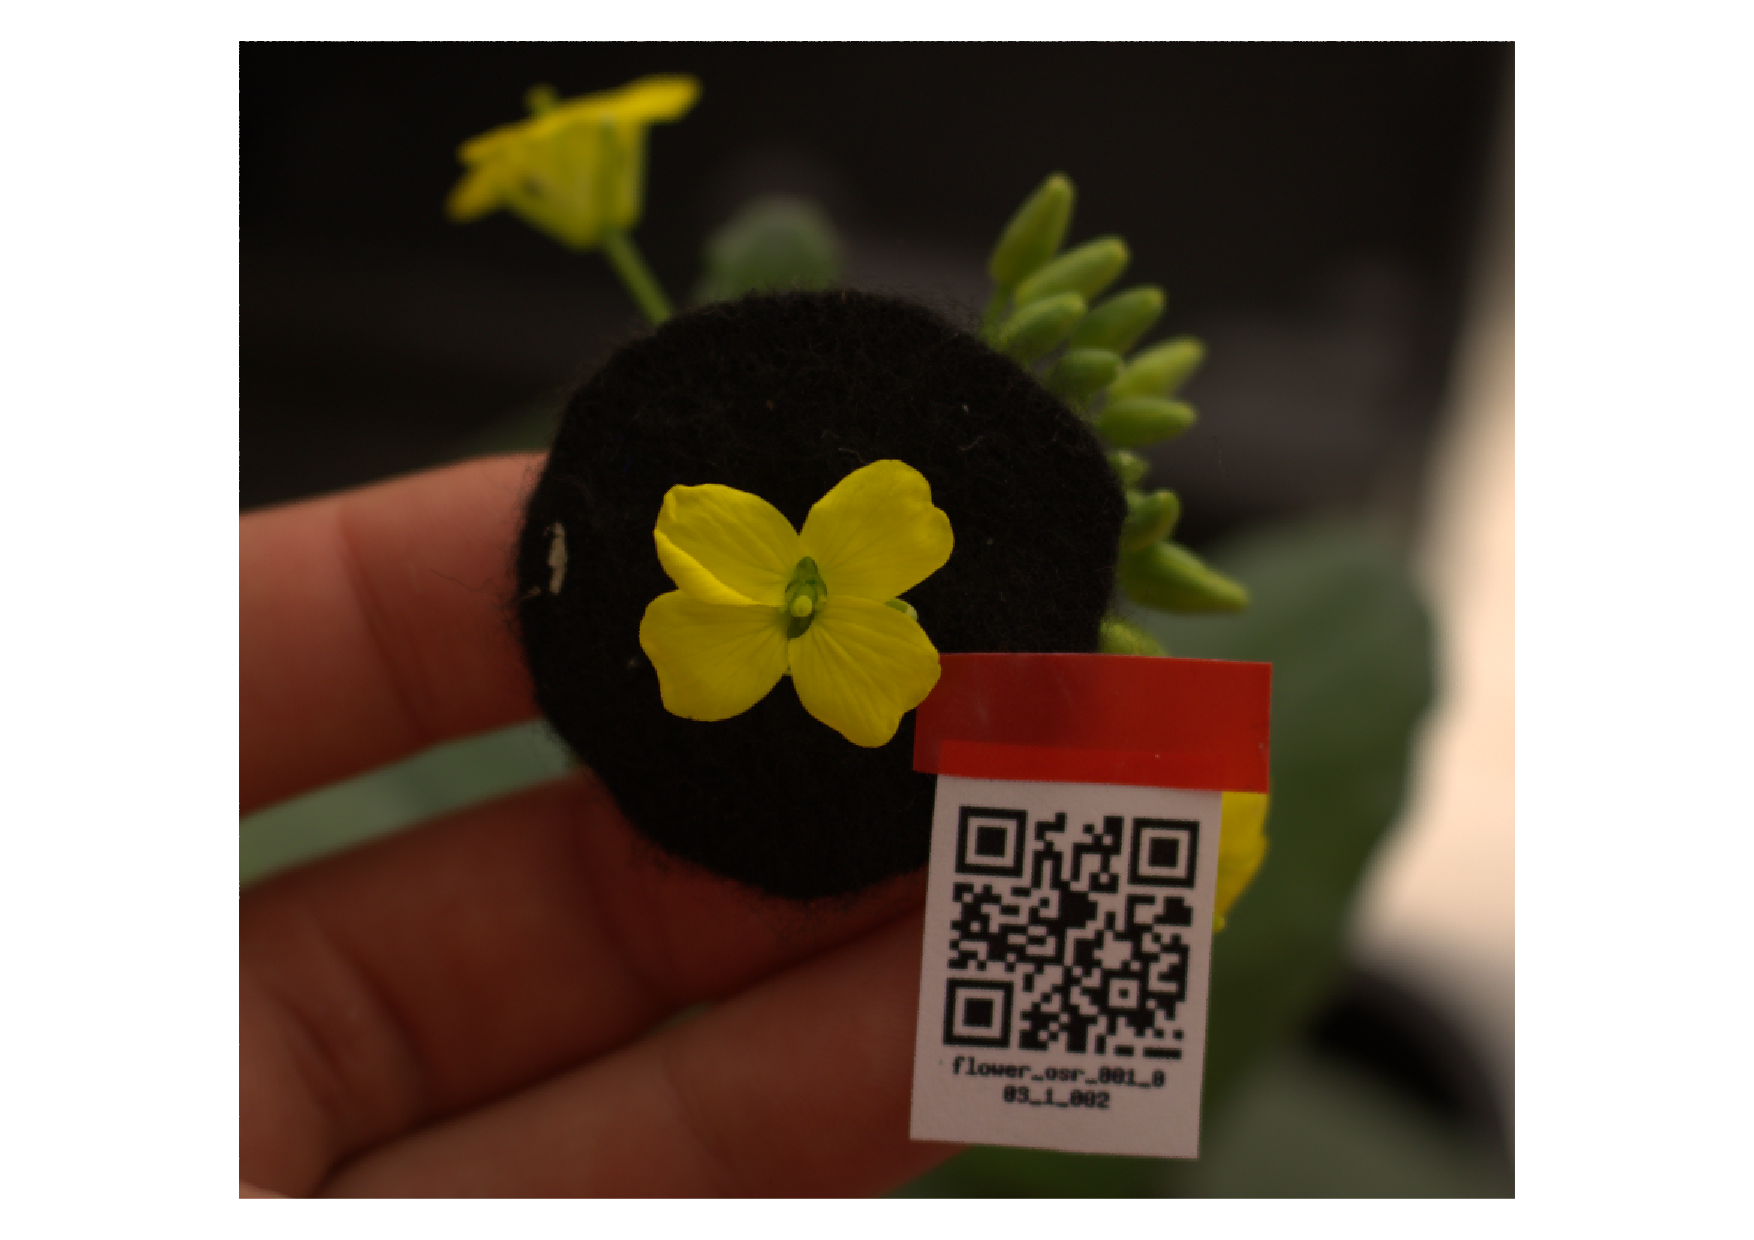
\includegraphics[width=0.9\linewidth]{origin}
		\caption{Original Image}
		\label{origin}
	\end{minipage}
	\centering
	\begin{minipage}{0.3\linewidth}
		\centering
		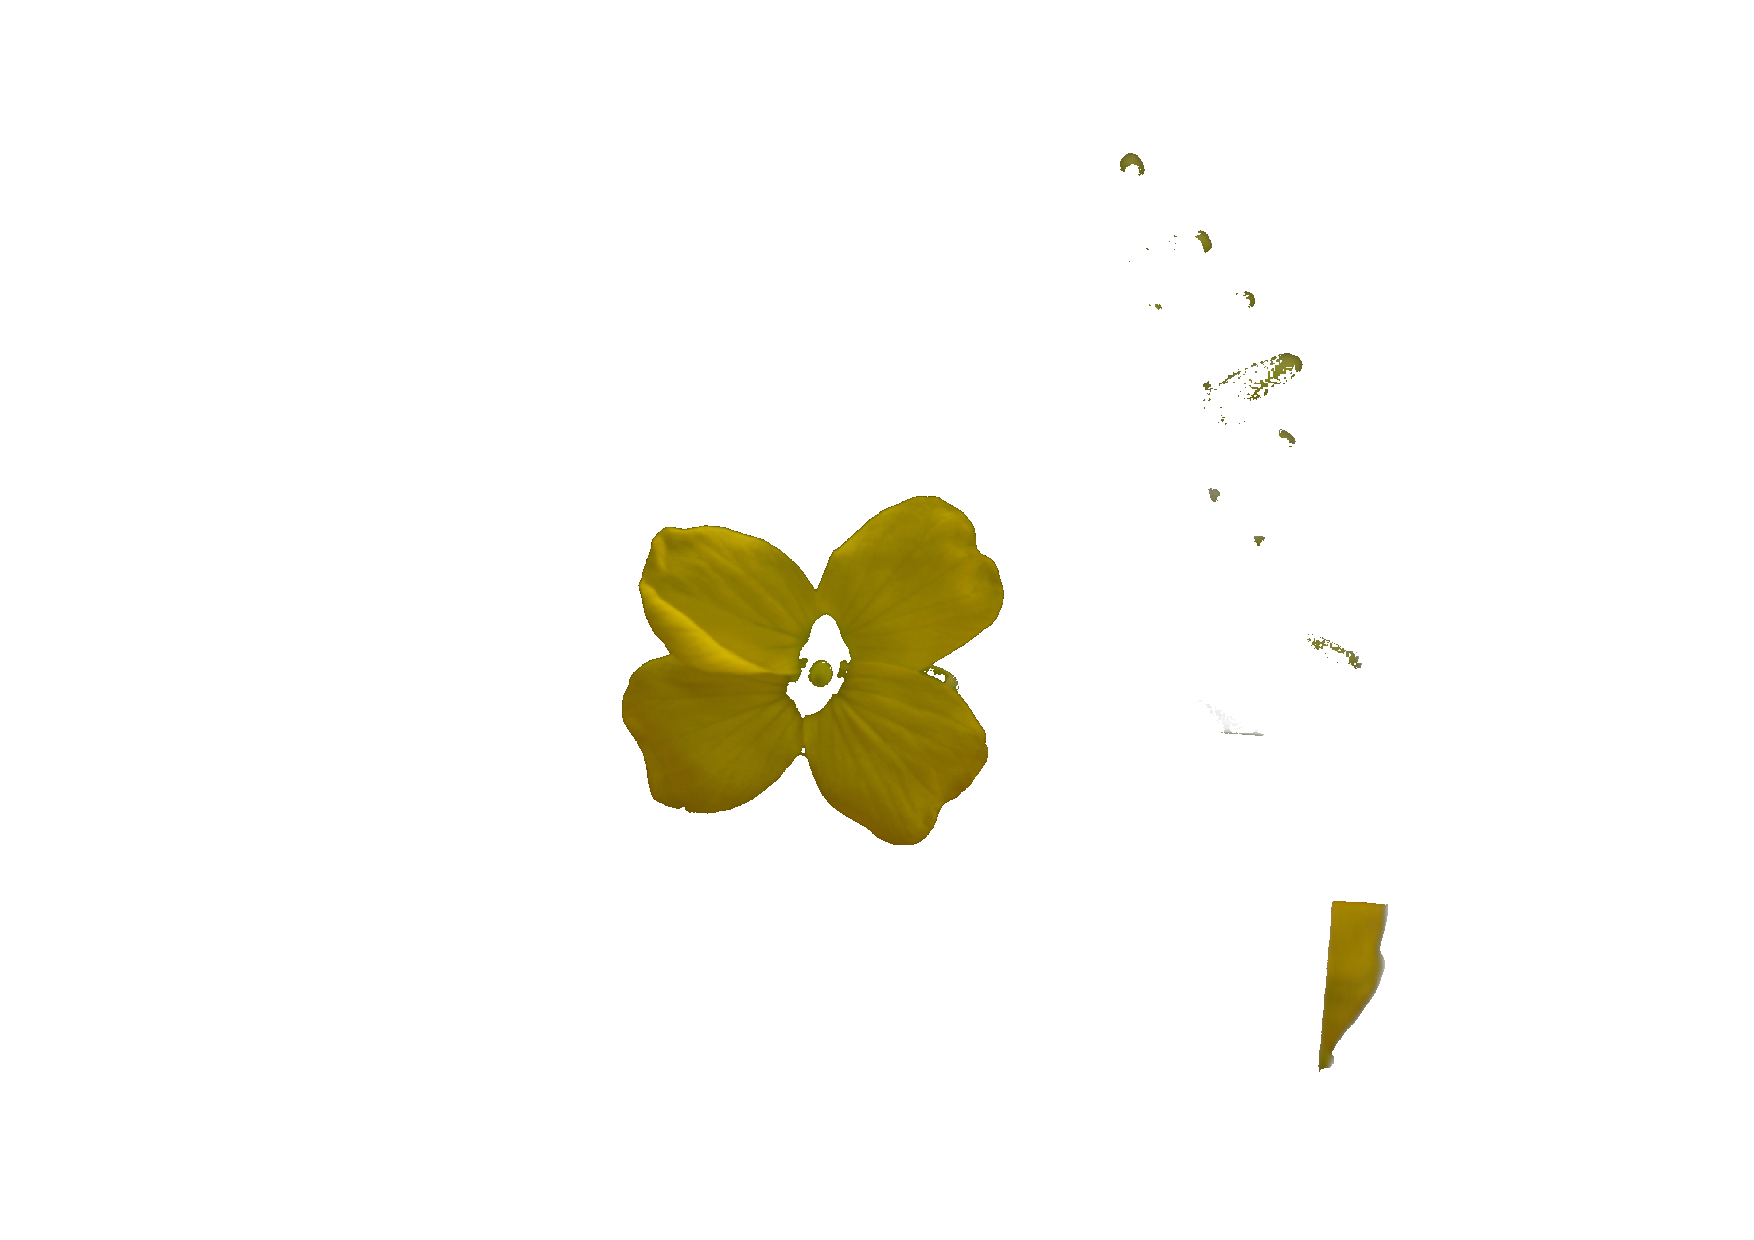
\includegraphics[width=1.2\linewidth]{automatic}
		\caption{Automatically processed}
		\label{automatic}
	\end{minipage}
	\centering
	\begin{minipage}{0.3\linewidth}
		\centering
		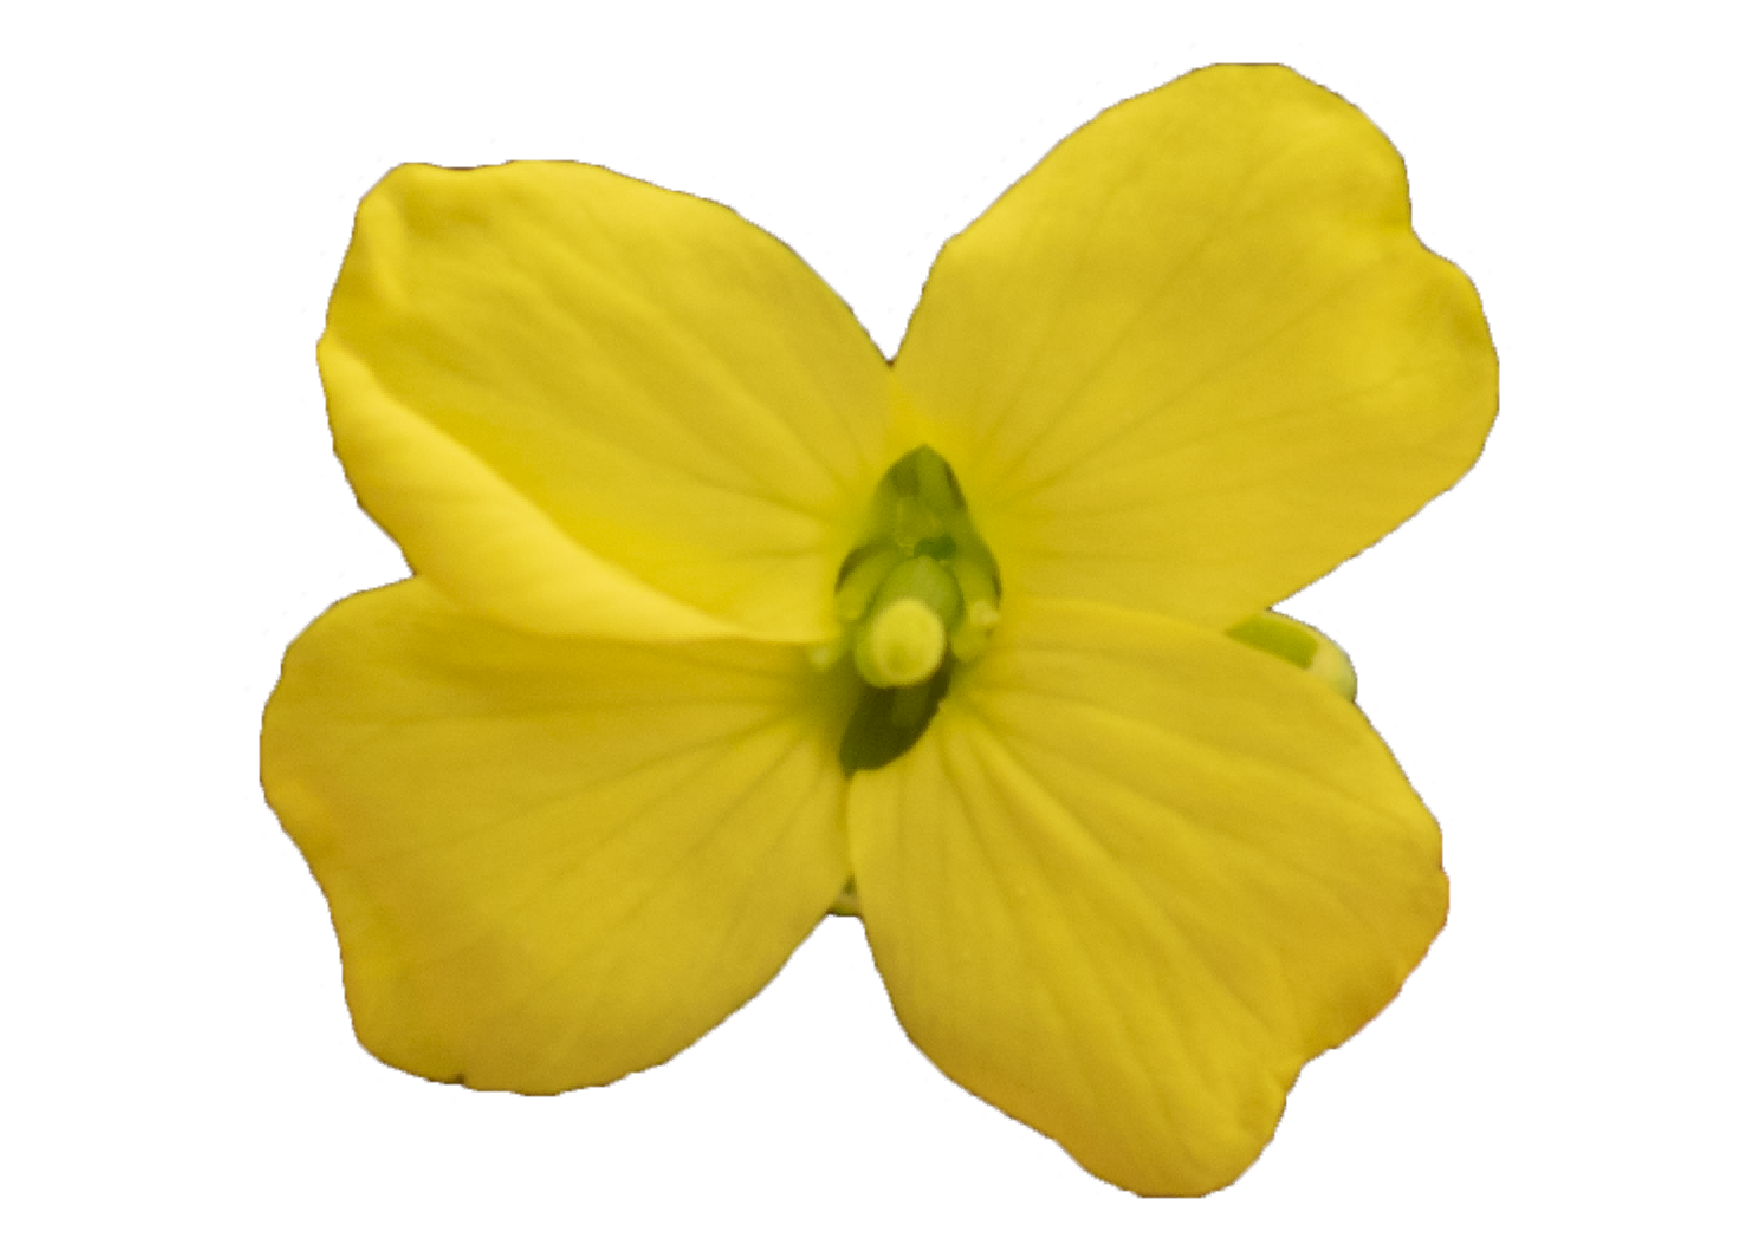
\includegraphics[width=0.6\linewidth]{hand}
		\caption{Manually processed}
		\label{manual}
	\end{minipage}
	\caption{Image segmentation of rape flowers}
	\label{fig:image-segmentation-of-rape-flowers}
\end{figure}


\subsection{Model}

\textbf{CNN}.
CNNs are feed-forward neural networks that consist of input, convolutional, pooling, fully connected, and output layers. It is a type of neural network that is specifically designed to process data in a grid-like manner.
As CNNs use convolutional operations to compute, their computational speed significantly exceeds the computational speed of general matrix operations. By combining convolutional layers with pooling layers, CNNs can effectively extract local features from data and reduce the dimensionality of local features by effectively extracting local features. By sharing weights, the number of weights can be reduced and the complexity of the model can be reduced.\par

\textbf{ResNet}.
ResNet is a deep residual network proposed by \citet{he2016deep}. Traditional CNNs propagate information from the input to the layers, resulting in vanishing gradients that make deep neural networks difficult to train. In order to solve this problem, ResNet adds blocks of residuals, each of which contains multiple convolutional layers as well as a $shortcut connection$ across layers, making it possible to move directly from a previous layer to a later one.
In this way, the network is easier to train and performs better in the area of image recognition. ResNet-50, which was used in this project, is a convolutional neural network with 50 layers and shows improved training and testing errors compared to other convolutional neural networks.

\textbf{LSTM}.
It is a type of recurrent neural network (RNN) that is designed to overcome some of the limitations of traditional RNNs when dealing with long-range dependencies or vanishing or exploding gradients.
As with standard RNNs, LSTMs have inputs and outputs for each hidden layer node, but they incorporate gated units to control information flow within their hidden layer nodes,the structure shows below Figure~\ref{LSTM}:

\begin{figure}[ht]
	\centering
	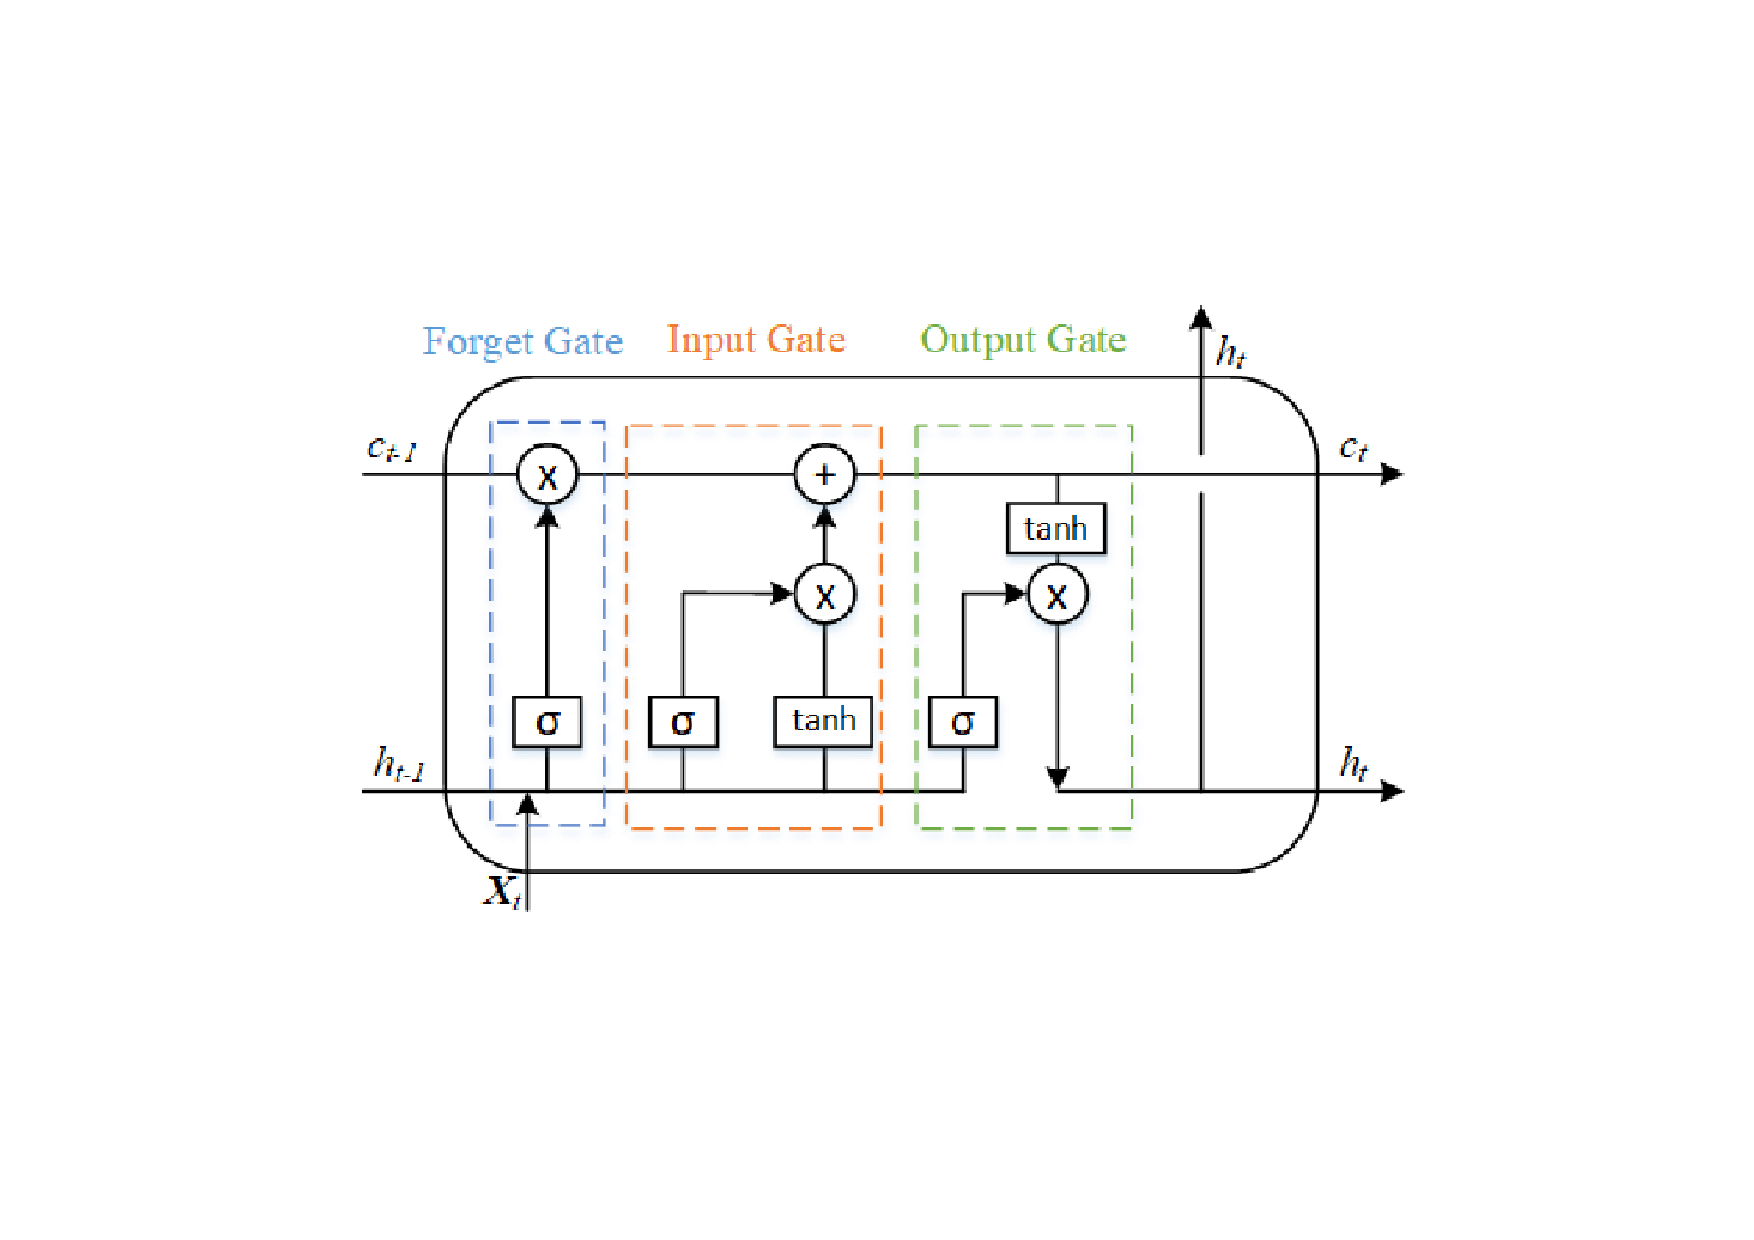
\includegraphics[scale=0.4]{LSTM-cell-according-to-Hochreiter-and-Schmidhuber-1997}
	\caption{The LSTM cell according to \citet{app122412980}}
	\label{LSTM}
\end{figure}

With the help of gating, new information can be selectively added and the previously accumulated information can be forgotten.
In this study, image changes in canola flowers change with pollination time. Therefore, LSTM was chosen to assist in acquiring time-series features to make the model more accurate.

\textbf{CNN-LSTM}.
Convolutional Neural Networks (CNNs) are known to perform very well on tasks involving the analysis or discovery of specific features and shapes in images, while Long Short-Term Memory (LSTM) Neural Networks perform very well on tasks involving temporal dimensions (e.g., time-series prediction) and sequences of data (e.g., sequences of images, sequences of signals over a specific time range, etc.).
This is mainly due to their ability to learn long-term dependencies in data. Since the images of rapeseed flowers in this project are constantly changing as pollination time passes, this architecture combining convolutional and LSTM layers can predict the next image in a series of images, dramatically improving classification accuracy and reasonableness.
The structure of multi-feature sequence classification CNN-LSTM model is shown in Figure~\ref{CNN-LSTM}. It mainly consists of signal input layer, CNN convolutional layer, pooling layer, LSTM layer and classification output layer. The CNN-LSTM based multi-input sequence classification task process is as follows:

\begin{figure}[ht]
	\centering
	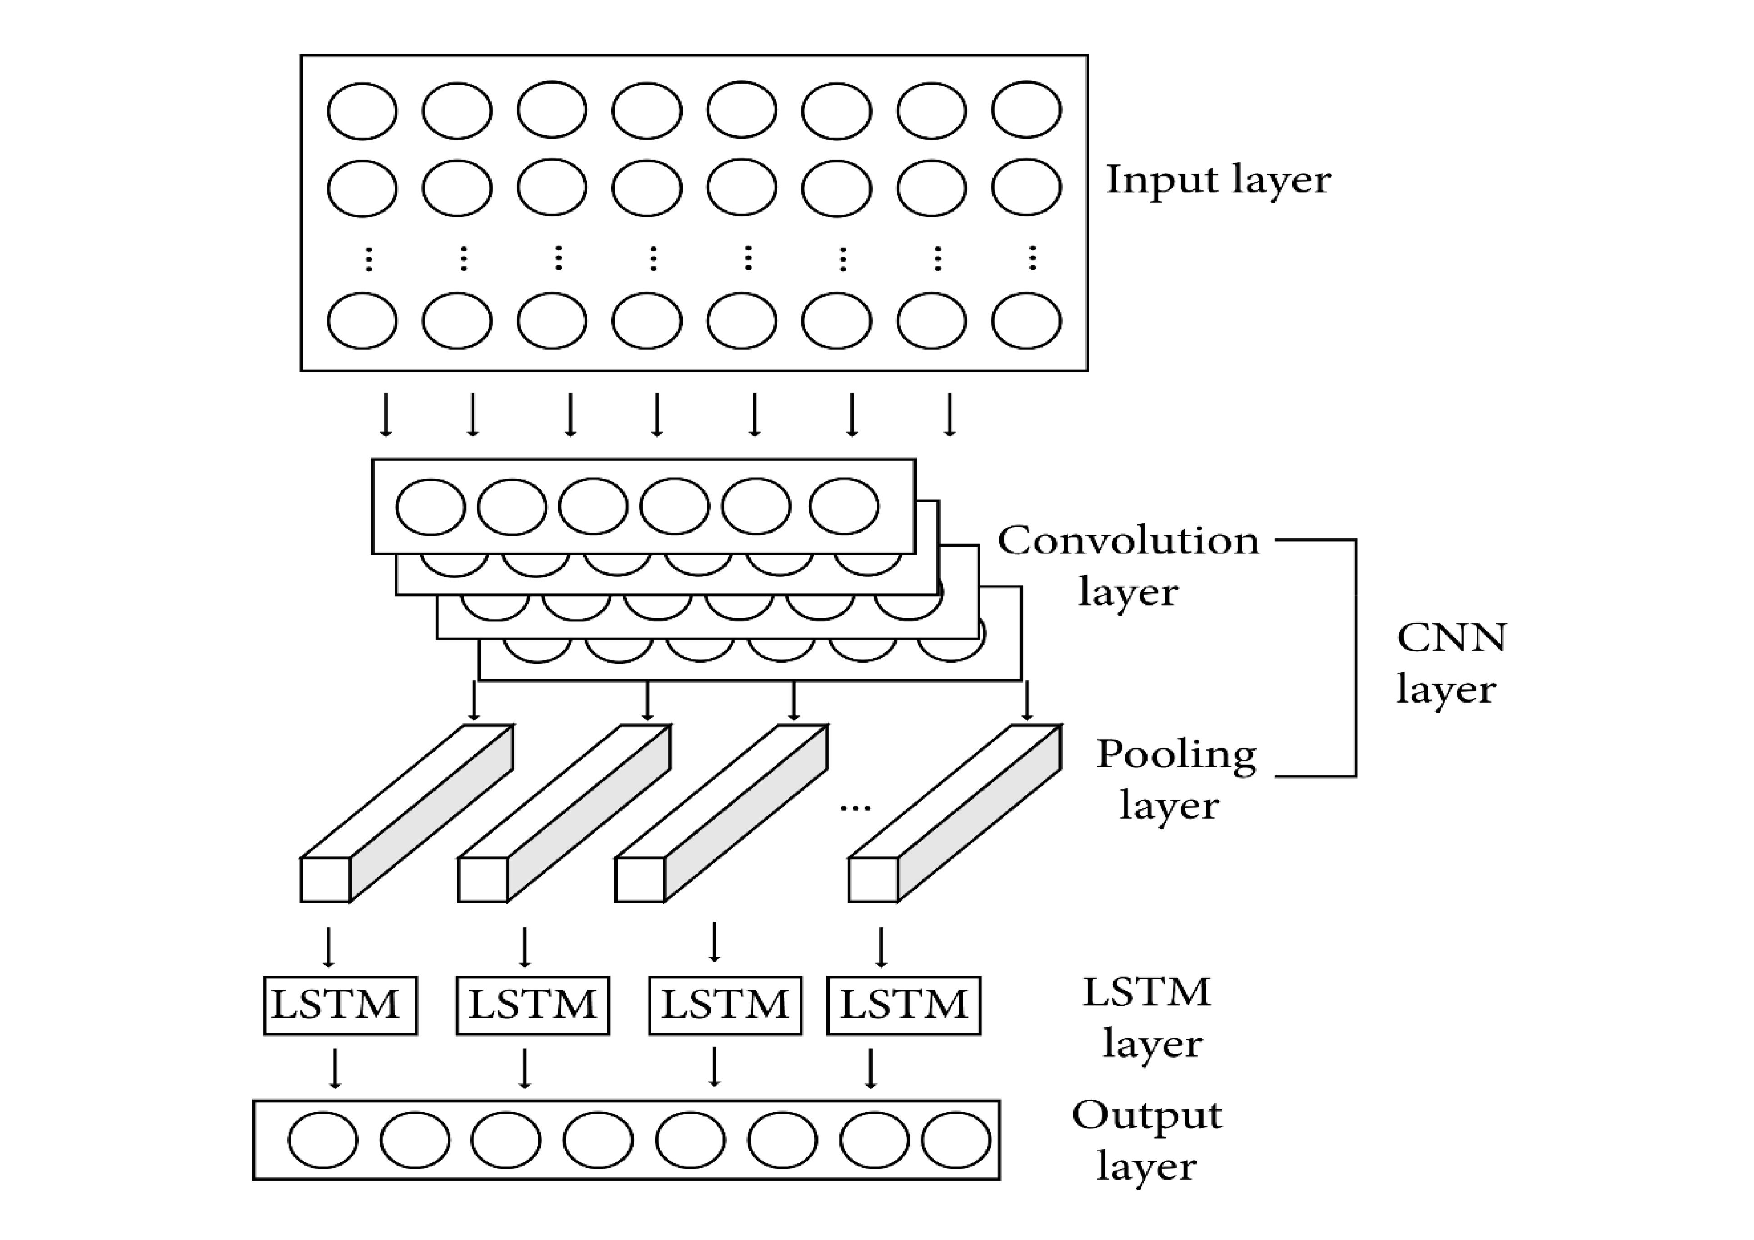
\includegraphics[scale=0.4]{CNN-LSTM}
	\caption{The structure of CNN-LSTM model \citet{inproceedings}}
	\label{CNN-LSTM}
\end{figure}

(1) The input signal is normalised and fed into the CNN convolutional layer, and features are adaptively extracted using the convolutional kernel;
(2) The extracted features undergo a pooling operation in the maximum pooling layer to reduce the data dimensionality and retain the main feature information;
(3) The dimensionality-reduced feature data is then used as the feature input to the LSTM layer to train the neural network and automatically learn sequence features;
(4) Use Adam's algorithm to back-propagate the training error and gradually update the model parameters layer by layer;
(5) Using the activation function, the signal features are classified to complete the classification task of multi-feature input sequences.

\subsubsection{Model evaluation}
It is important to note that there is no significant difference in the amount of data collected between the experimental and control groups in this project. Due to the fact that this is a binary classification problem with relatively balanced data, the accuracy can be used as an indicator of a model's performance.
Accuracy is the ratio of the number of correctly classified predictions to the total number of predictions; the higher the accuracy, the better the classifier.
There are two total categories of samples in a binary classification problem: Positive and Negative.The results of these classifications are categorised as follows:
(1) True Positive (TP): Successfully predicts positive samples as positive.
(2) True Negative (TN): Successfully predicts a negative sample as negative.
(3) False Positive (FP): incorrectly predicts a negative sample as positive.
(4) False Negative (FN): incorrectly predicts a positive sample as negative.

In a binary classification model, accuracy is defined as follows:
$$
Accuracy = {\frac{TP+TN}{TP+FP+TN+FN}}
$$

\subsubsection{Configurations}
The classification model is based on CNN-LSTM implemented by Pytorch \citep{paszke2019pytorch}. The output result of the CNN model is used as the input of the LSTM, and a fully connected layer is added after the LSTM layer to output the final result.

The backbone is pre-trained model ResNet-50, the optimal weight will be adjusted during the continuous training of the model, and the optimal model will be saved after the training.


\begin{table}[H]
\centering
\caption{Configurations of the classification task}
\begin{tabular}{lc}
\hline
Parameter & Value\\
\hline
Number of classes & 2\\
Backbone & ResNet-50\\
Images per batch & 4\\
Initial learning rate & 3e-05\\
number of epochs & 20\\
Augmentation & ResizeShortestEdge, RandomFlip, RandomAffine\\
\hline
\end{tabular}
\label{tab:classification}
\end{table}

Numpy 1.24.3 was used for data pre-processing. This part of classification model was implemented by Python 3.10, torch 1.13.

\section{Result}

\subsection{Model evaluation}
As the model has been pre-trained, the best model weights can be loaded at the beginning. To prevent overfitting, 20 percent of the data is extracted at a time for training, while the remainder is used for testing. The accuracy of the model is already high after seven epochs of training, but the loss still has room for improvement. Therefore, we decided to reduce the learning rate by half to 1.5e-05 in order to continue training. It has taken 14 epochs for the train loss to decrease to around 0.13, at which point the model accuracy has reached 0.96. To further reduce the loss, we reduced the learning rate by half to 7.5e-06, at which point the model performance stabilized. The loss (Figure \ref{Loss}) and accuracy (Figure \ref{Accuracy}) curves of the model are shown in the figures below:

\begin{figure}[htbp]
\centering
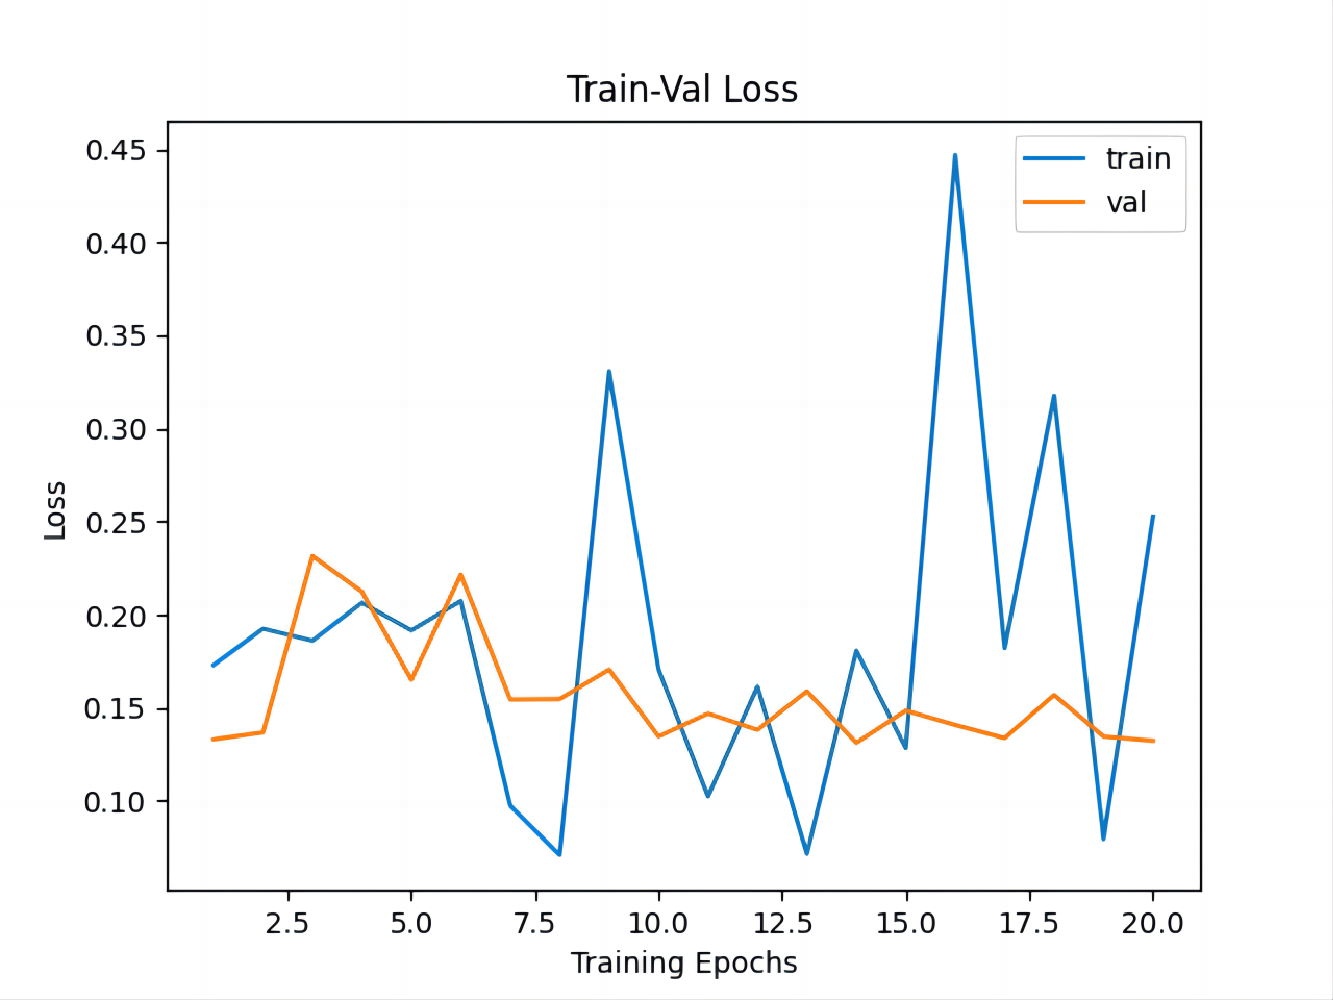
\includegraphics[scale=0.5]{Figure_1}
\caption{Loss curve:val\_loss is the loss value on the validation set, train\_loss is an error on the training set}
\label{Loss}
\end{figure}

\begin{figure}[htbp]
\centering
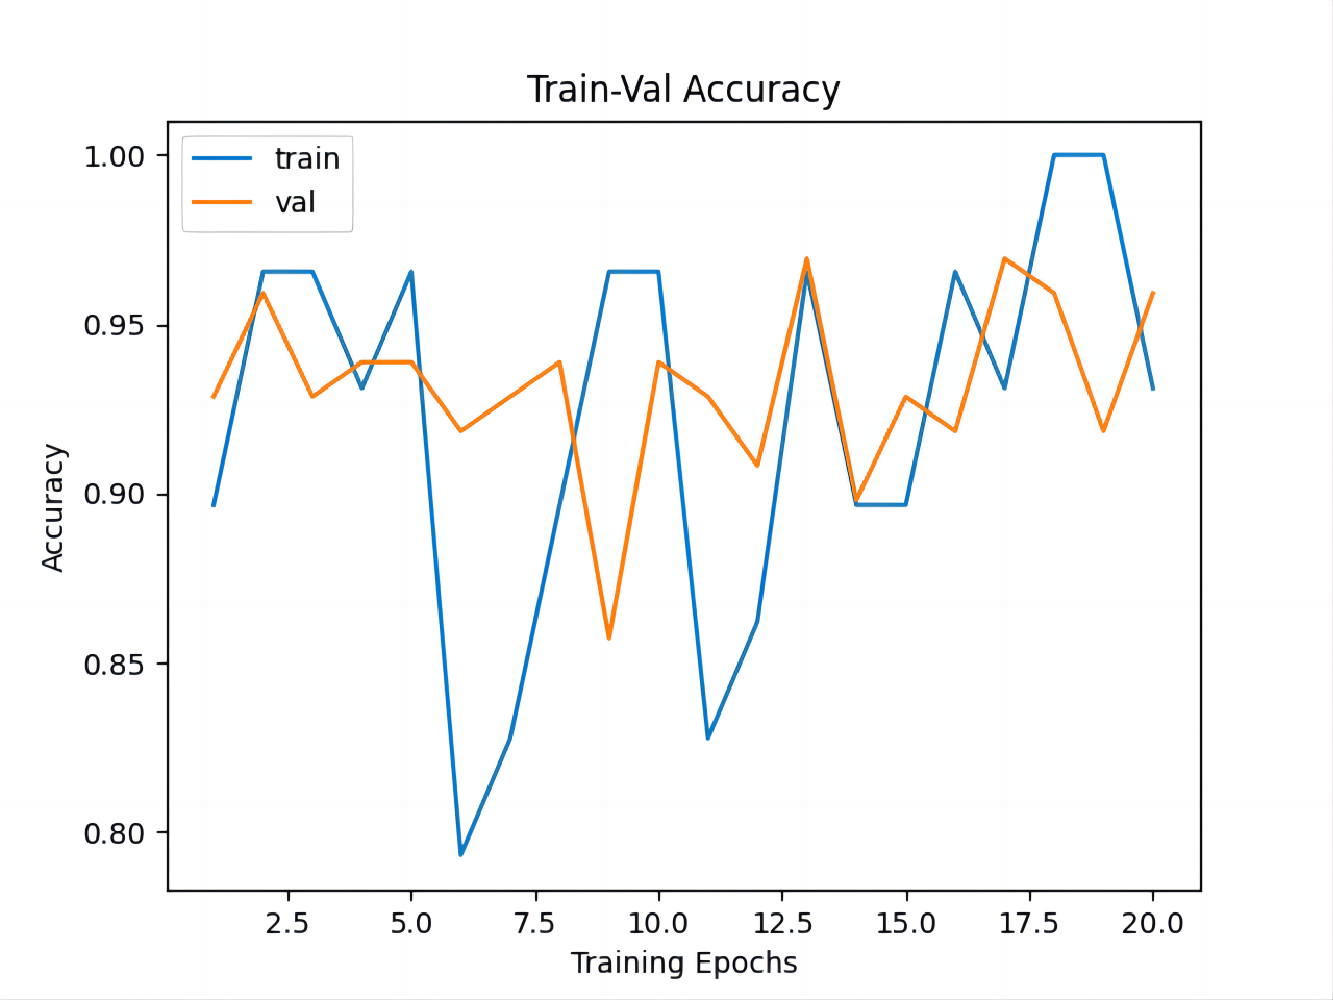
\includegraphics[scale=0.5]{accuracy}
\caption{Accuracy curve: val\_acc is the accuracy on the validation set, train\_acc is the accuracy on the training set}
\label{Accuracy}
\end{figure}


\subsection{Model application}
Once the classification model has been trained, it is applied to the full dataset to determine if it is capable of correctly predicting images in real-life situations. As with model training, the images are first augmented with data and then normalized to ensure consistent data input. It was necessary to classify the data at the time of input in order to determine the recognition rate at the moment of each monitoring (as mentioned, every four hours, over a 12-hour day), and the images were grouped into groups 1-10 based on the time of the monitoring, and due to the wilting of most of the flowers after the 7th monitoring, the amount of data in groups 8-10 was relatively small, but still of value as a reference, the result shows below:

\begin{table}[H]
\centering
\caption{Model prediction result}
\begin{tabular}{|l|l|l|}
\hline
Day & Monitoring Time point & Accuracy\\
\hline
1 & 1 & 0.7480\\
1 & 2 & 0.8028\\
2 & 3 & 0.7976\\
2 & 4 & 0.9412\\
2 & 5 & 0.8814\\
3 & 6 & 0.9070\\
3 & 7 & 0.8333\\
3 & 8 & 1.0000\\
4 & 9 & 1.0000\\
4 & 10 & 1.0000\\
\hline
\end{tabular}
\label{tab:prediction}
\end{table}

In (Table\ref{tab:prediction}), Time1 indicates when pollination was not done and it was pollinated after the first monitoring was completed. For the experimental group, Time2 indicates the second pollination and the control group was never pollinated. That is, two pollinations were carried out on the first day, and monitoring was carried out every 4 hours thereafter, monitor time indicates the number of times monitoring was actually carried out, Each flower was tested from opening until petal drop (approx. 3 days), so the first 6 times tested were the ones that were the most effective, after that, the model was affected due to the wilting of the flowers.

\subsection{Result analysis}
As far as the accuracy of the model predictions is concerned, the results are very promising. The model's accuracy at predicting that an image is not pollinated is the first indicator of accuracy when not pollinated. The prediction accuracy at the time of pre-pollinated does not have much meaning since there is no difference between the experimental group and the control group. In other words, in the first time-step, none of the flowers were pollinated, indicating that the accuracy of the model in predicting that none of the flowers were pollinated was 0.7480. As a result of the second monitoring time, when the experimental group is pollinated and the control group is not, the accuracy of the model prediction is about 0.8 at this point, which is already a high number, however it is not sufficient for practical application. At the fourth time point, recognition rates increase significantly, which, from a biological perspective, could be due to the intrinsic biosignaling of the flower. Due to the fact that the LSTM relies on data from the last four moments to make predictions, the fourth time-steps will have more data and will be more accurate than the first three moments.
After the 5th and 6th time-steps, the prediction accuracy is approximately 0.9 with a slight decrease in accuracy. This is caused by the flowers gradually starting to fade, so that the biological signal is no longer significant. At the beginning of the 7th moment, the flowers basically withered and the prediction accuracy decreased. Although the final model accuracy was 1, the flowers had faded and were no longer meaningful for identifying whether pollination was occurring. So it follows that the best time to apply the model is at time 4, the third monitoring time after pollination. Extending this to the general case, monitoring at the 8th hour after pollination is meaningful for detection, and the highest identification accuracy is obtained around the 20th hour after pollination. In conclusion, the classification model The classification model itself has an accuracy of 0.96, and the fourth time-point is the best recognition point for detection.


\section{Discussion}
Some studies\citep{reif2008analysis} have shown that changes in spectral reflectance are a biosignal that can identify whether a plant has been pollinated, but the measurement of spectral reflectance requires specific instrumentation, which makes it easier to obtain information from RGB images. Therefore, this project aims to achieve a non-invasive examination of pollination in rape flowers by developing a machine-learning tool to extract information from RGB images in order to obtain pollination senescence signals. The results of my project show that contemporary machine learning and artificial intelligence techniques can be widely used in the field of computer vision, which is feasible and practically valuable for RGB image feature extraction to achieve classification, and that computer vision techniques can discover microscopic signals in flower petals that cannot be observed by the naked eye.

This project uses a hybrid deep neural network model (CNN-LSTM) as its machine learning algorithm. In both experimental and control groups, canola flowers fade over time, regardless of whether they have been pollinated or not. One advanced goal of this project is to determine when rape flowers have been pollinated. CNNs are excellent at identifying image features, but they cannot account for changes in the time dimension. LSTMs, on the other hand, can remember and selectively forget data over time and are capable of retrieving information from a period of time-series data. For the purposes of constructing this model, the spatio-temporal dimensions acquired by the CNN are used as inputs to the LSTM, and the image features from every four moments are used as a set of data inputs and are sequentially pushed backwards as inputs.

According to the conclusions of the tests, at the fourth moment, on the second day, the model predicted pollination with an accuracy of 0.94. The main reason for this increase in accuracy compared to the first three moments, which hovered around 0.80, is that every fourth moment of the image was used as a set of inputs when training the data, so that the fourth moment could already be used as an observation to monitor the biosignal. The predictive accuracy of the model then decreases at moments 5-7, the underlying reason being that canola flowers age rapidly after pollination, withering faster compared to unpollinated canola flowers, and images of flowers in the senescent phase are not easily recognisable. Most of the flowers in the 8th-10th moments have already withered and only a small portion of the dataset is retained in the image, therefore the model overfits at this stage and although the recognition accuracy reaches 1, this stage should not be used as a basis for judgement.

Through this project, we developed a trained classification model for identifying whether an RGB image of rape flower is pollinated or not, with excellent accuracy as well as robustness. Nevertheless, based on the underlying logic of deep learning, this project still has room for improvement or optimization:

Firstly, regarding the dataset, which is derived from greenhouse-grown rape flowers. Due to the fact that the plants are planted by hand, the total number of plants is limited. Moreover, the flowering period after pollination of rape flowers is very short and the cultivation cycle is long, resulting in a small number of samples in the dataset. As a result, there is a tendency for the model to exhibit overfitting problems, which may have a negative impact on the model's ability to generalize. It is also worth mentioning that, unlike spectral analyses of plants, RGB images are very much affected by the environmental conditions at the time of shooting. For example, the intensity of light, the angle of the camera, parameter settings, etc., all of these can have a dramatic effect on the visual quality of the image.

Besides, in terms of image segmentation, this project tried both automatic and manual segmentation. There are advantages and disadvantages to both methods. The use of script-based automatic segmentation will affect recognition accuracy in some background image clutter, whereas the use of manual segmentation is highly accurate but time-consuming and difficult to process a large amount of data.

It is possible to find solutions to all the above problems. And it is possible to feed a large amount of image data into the model for training in order to make the model more pervasive, resulting in an improvement in the model's ability to recognize and monitor multiple species in practical applications. For the clarity of the images themselves as well as the quality of the images, it is possible to develop and equip appropriate whole-plant phenotyping equipment to enable semi-automatic or even fully-automatic input. Biological, engineering and other disciplines will be used to automate and standardize the monitoring process. By applying scripts, the accuracy of image segmentation can be increased accordingly without interfering with the image input.

All in all, this project holds great promise for agricultural applications, achieving high-accuracy non-invasive identification of pollination. This model can be combined with engineering equipment to realize the application of automation.



\newpage

\section*{Data and code availability}
All data and code in this project are available from \href {https://github.com/Midsummer874/CMEECourseWork/tree/master/MScProject} {MSc project github}



\bibliographystyle{agsm}
\bibliography{reference.bib}
\pagebreak

\section*{Supplementary Information}

\begin{figure}[ht]
	\centering
	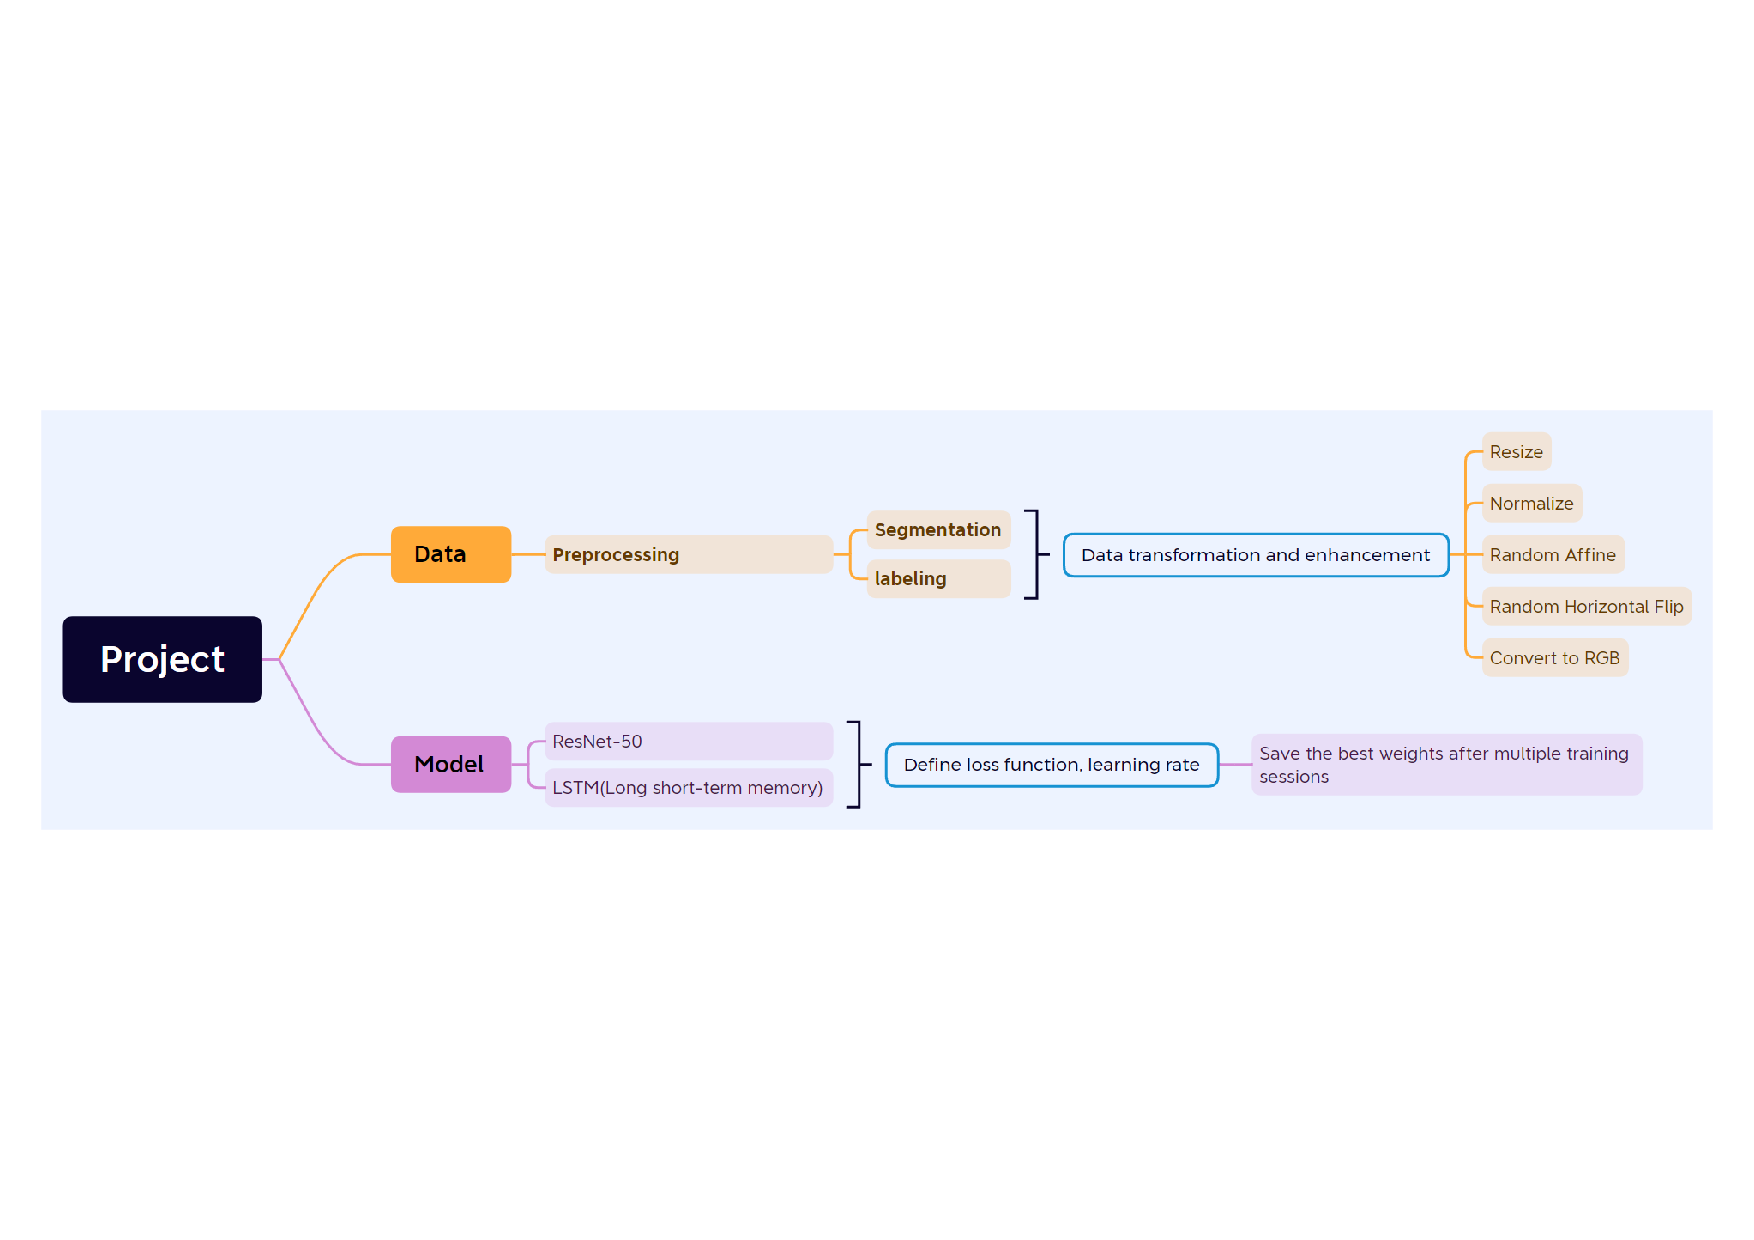
\includegraphics[scale=0.4]{workflow.pdf}
	\caption{Workflow of the project}
	\label{workflow}
\end{figure}

\end{spacing}
\end{document}